%************************************************
\chapter{Algoritmo seleccionado: Statistical Dependency Analysis With Support
  Vector Machines}
\label{ch:algorithm}
%************************************************

\citeauthor{yamada2003} \cite{yamada2003} proponen un método para analizar las
dependencias palabra-a-palabra mediante una estrategia \emph{bottom-up} -- de
abajo a arriba. -- Para ello se hace uso de la técnica de \ac{AA}
\acfi{SVM}. Sus experimentos se basan en árboles de dependencias creados a
partir del corpus \ac{PTB}, logrando una precisión superior al 90\% para
dependencias palabra-a-palabra. Aún siendo esta precisión inferior al
\nameref{sec:stateoftheart}, hay que tener en cuenta que este método no utiliza
información sobre la estructura de las frases.

El tipo de anotaciones usadas en este método pueden verse en la
\autoref{fig:deptree}. Esta forma de ilustrar las dependencias palabra-a-palabra
es más sencilla de entender para los anotadores que el usual estilo \ac{PTB} ---
\autoref{fig:strtree} --- El problema del estilo \ac{PTB} es que requiere que
los anotadores tengan un ámplio conocimiento de la teoría lingüística del
idioma, así como de la estructura de las frases, además del dominio específico
que trata el problema. Como ventaja adicional, la representación del árbol de
dependencias de la \autoref{fig:deptree} hace que la construcción de los datos
de entrenamiento sea menos ruidosa, al ser el proceso de anotación más simple.
\begin{figure}[ht]
%\resizebox{1.3\textwidth}{!}{%
\tiny
\begin{tikzpicture}[every node/.style={align=center}]
  \tikzset{
    edge from parent/.style={
      draw,edge from parent
      path={(\tikzparentnode.south)-- +(0,-8pt)-| (\tikzchildnode)}
    },
    frontier/.style={distance from root=208pt}, % Align leaf nodes
    level 1+/.style={level distance=18pt} % Distance between levels
  }

   \Tree [.S
             [.NP Rolls-Royce\\NNP Motor\\NNP Cars\\NNPS Inc\\NNP ]
             [.VP said\\VBD
                [.SBAR [.none ]
                   [.S
                      [.NP it\\PRP ]
                      [. VP expects\\VBZ
                         [.S
                            [.NP its\\PRP\$ U.S\\NNP sales\\NNS ]
                            [.VP to\\TO
                               [.VP remain\\VB
                                  [.ADJP steady\\JJ ]
                                  [.PP at\\IN
                                     [.NP
                                        [.QP about\\IN 1200\\CD ]
                                        cars\\NNS
                                     ]
                                  ]
                               ]
                            ]
                         ]
                      ]
                   ]
                ]
             ]
         ]
\end{tikzpicture}
%}
\caption{Estructura en árbol de la frase ``Rolls-Royce Motor Cars Inc. said it
  expects its U.S. sales to remain steady at about 1,200 cars.''}
\label{fig:strtree}
\end{figure}
\begin{figure}[th]
  \scriptsize
  \begin{tikzpicture}[every node/.style={align=center},level distance=30pt]
    \tikzset{edge from parent/.append style={<-, >=latex,thick}}
   \Tree [.said\\VBD 
             [.Inc.\\NNP Rolls-Royce\\NNP Motor\\NNP Cars\\NNPS ]
             [.expects\\VBZ it\\PRP
                [.remain\\VB
                   [.sales\\NNS its\\PRP\$ U.S\\NNP ]
                   to\\TO
                   steady\\JJ 
                   [.at\\IN [.cars\\NNS [.about\\IN 1200\\CD ] ] ]
                ]
             ]
           ]
   \end{tikzpicture}
   \caption{Árbol de parseo de dependencias}
   \label{fig:deptree}
\end{figure}
En la estructura propuesta por \citeauthor{yamada2003} se realiza un análisis
estadístico de las dependencias de un idioma. Para lograr este análisis, se usa
la técnica de aprendizaje conocida como \ac{SVM}, ya que es capaz de tratar con
espacios de características a gran escala. En los siguientes párrafos se hará
una breve intoducción a esta técnica.

\section{Una introducción a las SVMs}
\label{sec:svmintro}

\nocite{yaser2012} Los modelos lineales son muy poderosos, mediante
transformaciones lineales es posible incrementar en gran medida su capacidad
expresiva. Sin embargo, incrementar dicha capacidad tiene un precio, el sobre
ajuste y más tiempo de cómputo. \ac{SVM} usa un cojín de seguridad cuando separa
los datos. Este cojín logra que la \ac{SVM} sea más robusta al ruido, reduciendo
así el sobre ajuste. Además, \ac{SVM} es capaz de trabajar con la herramienta
conocida como \emph{kernel} --- la cual permite operar de forma eficiente con
transformaciones no lineales de gran dimensión ---. Estas dos características --
el cojín de seguridad y el \emph{kernel} -- hacen de la \ac{SVM} un modelo no
lineal muy robusto y potente con regularización automática. Las \ac{SVM} son muy
populares por su facilidad de uso y su buen rendimiento.

\ac{SVM} usa la estrategia del máximo margen ideada por
\emph{Vapnik}. Supongamos $l$ datos de entrenamiento
$(\mathbf{x}_i,y_i), (1 \leq i \leq l)$, donde $\mathbf{x}_i$ es un vector de
características en un espacio de dimensionalidad $n$, $y_i$ es la etiqueta de la
clase $\{-1, +1\}$ de $\mathbf{x}$. Las \acp{SVM} encuentran un hiperplano
$\mathbf{w}\cdot \mathbf{x} + b = 0$ que separe correctamente los datos de
entrenamiento de forma que tengan margen máximo, es decir, con la máxima
distancia entre dos hiperplanos $\mathbf{w}\cdot \mathbf{x} + b \geq 1$ y
$\mathbf{w}\cdot \mathbf{x} + b \leq -1$, como se aprecia en la
\autoref{fg:svmexample}
\begin{figure}[ht]
  \centering
  \missingfigure{SVM example}
  \caption{Ejemplo \ac{SVM}}
  \label{fg:svmexample}
\end{figure}
El uso de \ac{SVM} para el análisis estadístico de dependencias presenta
principalmente dos ventajas. La primera de ellas es un gran poder de
generalización en espacios de características de grandes dimensiones. Segunda,
gracias al \emph{kernel trick} es posible entrenar al modelo para que aprenda a
partir de la combinación de múltiples características.

Para poder trabajar con clasificaciones no lineales uno de los \emph{kernels}
posibles es el polinomial -- $(\mathbf{x}` \cdot \mathbf{x}`` + 1)^d$ -- Con
este \emph{kernel} se habilita la posibilidad de tener en cuenta combinaciones
de $d$ características sin incrementar demasiado el tiempo de cálculo. En el
problema que nos ocupa, esto se traduce en la capacidad de entrenar reglas de
dependencias usando varias características, como \ac{POS} \emph{tags}, las
palabras en sí y sus combinaciones.

\section{Análisis de dependencias determinístico}
\label{sec:depanalysis}

\subsection{Acciones para el parseo}
\label{subsec:parseractions}

El trabajo de \citeauthor{yamada2003} propone tres acciones para construir el
árbol de dependencias. Es aquí cuando entra en juego la \ac{SVM}, ya que
aprenderá las acciones de los datos de entrenamiento y predecirá qué acciones
realizar para datos nuevos. El árbol de dependencias se construye de izquierda a
derecha, siguiendo la dirección de lectura habitual. Las tres acciones
posibles son \emph{Shift, Right} y \emph{Left} --- \textsc{Desplazar, derecha} e
\textsc{izquierda}. --- Estas acciones se aplican a dos palabras vecinas, nombradas a
partir de ahora nodos objetivo. Se pasa ahora a describir cada una de las
acciones.

\textsc{Desplazar} indica que no se ha realizado ninguna construcción en el
árbol de dependencias entre los nodos objetivo. La acción para esta situación
simplemente desplaza una posición a la derecha la ventana que apunta a los nodos
objetivo. En la figura \autoref{fig:shiftaction} muestra un ejemplo concreto.

\tikzset{
  notarget/.style={rectangle, rounded corners, minimum
    width=1cm, minimum height=1cm,text centered, draw=none,
    opacity=0,text opacity=.4,align=center},
  target/.style={rectangle, rounded corners, minimum width=1cm, minimum
    height=1cm,text centered, draw=black, very thick,text
    opacity=1,align=center}}
  
\begin{figure}[ht]
  \centering
  \begin{subfigure}[b]{0.3\textwidth}
    \begin{tikzpicture}[node distance=1.2cm]
      \node (n1) [notarget] {I\\PRP};
      \node (n2) [target, right of=n1] {saw\\VBD};
      \node (n3) [target, right of=n2] {a\\DT};
      \node (n4) [notarget, right of=n3] {girl\\NN};
      \draw [thick,->] (n4) -- ++(1cm,0);
    \end{tikzpicture}
    \caption{}
  \end{subfigure}
  \qquad\qquad
  \begin{subfigure}[b]{0.3\textwidth}
    \begin{tikzpicture}[node distance=1.2cm]
      \node (n1) [notarget] {I\\PRP};
      \node (n2) [notarget, right of=n1] {saw\\VBD};
      \node (n3) [target, right of=n2] {a\\DT};
      \node (n4) [target, right of=n3] {girl\\NN};
    \end{tikzpicture}
    \caption{}
  \end{subfigure}
  \caption{Ejemplo de la acción \textsc{Desplazar}. (a) muestra el
    estado antes de aplicar la acción. (b) el resultado trasaplicarla}
  \label{fig:shiftaction}
\end{figure}
\textsc{Derecha} construye una relación de dependencia entre los nodos
objetivo. De los dos nodos objetivo, el de la izquierda pasa a ser hijo
del nodo de la derecha. En la \autoref{fig:rightaction} puede observarse el
efecto de esta acción.
\begin{figure}[ht]
  \centering
  \begin{subfigure}[b]{0.4\textwidth}
    \begin{tikzpicture}[node distance=2mm]
      \node (n1) [notarget] {I\\PRP};
      \node (n2) [notarget, right=of n1] {saw\\VBD};
      \node (n3) [target, right=of n2] {a\\DT};
      \node (n4) [target, right=of n3] {girl\\NN};
      \node (n4') [target, right=of n4,draw=none,anchor=west] {};
      \node (n5') [target, below=5mm of n4',anchor=north,draw=none] {};
      \draw [thick,->] (n5'.center) -- ++(5mm,0);
    \end{tikzpicture}
    \caption{}
  \end{subfigure}
  \qquad\qquad
  \centering
  \begin{subfigure}[b]{0.4\textwidth}
    \begin{tikzpicture}[node distance=2mm]
      \node (n1) [notarget] {I\\PRP};
      \node (n2) [notarget, right=of n1] {saw\\VBD};
      \node (nn) [notarget,draw=none,right=of n2] {};
      \node (n3) [target, right=of nn] {girl\\NN};
      \node (n4) [target, below=5mm of n3] {a\\DT};
      \draw [thick,->] (n4) -- (n3);
    \end{tikzpicture}
    \caption{}
  \end{subfigure}
  \caption{Ejemplo de la acción \textsc{Derecha}. (a) Estado antes de la
    acción. (b) Estado tras aplicar la acción}
  \label{fig:rightaction}
\end{figure}
\textsc{Izquierda} construye una relación de dependencia entre los nodos
objetivo. De los dos nodos objetivo, el de la derecha pasa a ser hijo del nodo
de la izquierda. En la \autoref{fig:leftaction} se ilustra esta situación.
\begin{figure}[ht]
    \centering
  \begin{subfigure}[b]{0.3\textwidth}
    \begin{tikzpicture}[node distance=2mm]
      \node (n1) [notarget] {I\\PRP};
      \node (n2) [target, right=of n1] {saw\\VBD};
      \node (n3) [target, right=of n2] {girl\\NN};
      \node (n4) [notarget, below=5mm of n3,anchor=north] {a\\DT};
      \node (n4') [target,below=5mm of n4,draw=none] {};
      \node (n5') [target,right=of n4',draw=none] {};
      \draw [thick,->] (n4) -- (n3);
      \draw [thick,->] (n5'.center) -- ++(5mm,0);
    \end{tikzpicture}
    \caption{}
  \end{subfigure}
  \qquad\qquad
  \centering
  \begin{subfigure}[b]{0.3\textwidth}
    \begin{tikzpicture}[node distance=2mm]
      \node (n1) [notarget] {I\\PRP};
      \node (n2) [target, right=of n1] {saw\\VBD};
      \node (n4) [target, below=5mm of n2,anchor=north] {girl\\NN};
      \node (n3) [notarget, below=5mm of n4,anchor=north] {a\\DT};
      \draw [thick,->] (n4) -- (n2);
      \draw [thick,->] (n3) -- (n4);
    \end{tikzpicture}
    \caption{}
  \end{subfigure}
  \caption{Ejemplo de la acción \textsc{Left}. (a) Estado antes de la
    acción. (b) Estado tras aplicar la acción}
  \label{fig:leftaction}
\end{figure}

\subsection{Descripción del algoritmo}
\label{subsec:algdesc}

El Algoritmo~\autoref{algorithm:parsing} consiste de dos partes. Primero se
estima la acción apropiada usando la información contextual rodeando los nodos
objetivo. Segundo, se construye el árbol de dependencias ejecutando las acciones
estimadas en el primer paso.
\begin{algorithm}[H]
  \caption{Algoritmo de parseo}
  \label{algorithm:parsing}

  \algdef{SnE}{Init}{EndInit}{\textbf{Initialize:}}
  \algdef{snE}{Start}{EndStart}
  
  \begin{algorithmic}[1] % The number tells where the line numbering should start
    \State \textbf{Input Sentence:} $(w_1, p_1),(w_2,p_2),\cdots,(w_n,p_n)$
    \Init
       \State $i\gets 1$
       \State ${\cal T}\gets \{(w_1, p_1),(w_2,p_2),\cdots,(w_n,p_n)\}$
       \State $\text{no\_construction}\gets \text{true}$
    \EndInit
    \Start
       \While{$|{\cal T}| \geq 1$}
          \If{$i == |{\cal T}|$}
             \If{no\_construction == true}
                \textbf{break}
             \EndIf
             \State $\text{no\_construction}\gets \text{true}$
             \State $i\gets 1$
          \Else
             \State $\mathbf{x}\gets \text{getContextualFeatures(${\cal T}, i$)} $
             \State $y\gets \text{estimateAction(model, $\mathbf{x}$)}$
             \State construction(${\cal T}, i, y$)
             \If{$y == \text{\emph{Left} or \emph{Right}}$}
                $\text{no\_construction}\gets \text{false}$
             \EndIf
          \EndIf
       \EndWhile
    \EndStart
    \end{algorithmic}
\end{algorithm}
Cuando el algoritmo se ejecuta, la variable $i$ representa el índice del nodo de
la izquierda del par de nodos objetivos, $i + 1$ el de la derecha, dichos nodos
están en ${\cal T}$. ${\cal T}$ contiene la secuencia de nodos a los que se debe
estimar una acción, estos nodos se corresponden con los nodos raíz de los
árboles que se van construyendo a lo largo del proceso de parseado. Como es
lógico, inicialmente todos los nodos $t_i\in {\cal T}$ están compuestos
únicamente por la raíz, sin tener hijos. La información que guarda cada nodo es
el par $(w_i, p_i)$, donde $w_i$ es una palabra y $p_i$ su \ac{POS} \emph{tag}.

La estimación sobre qué acción aplicar se lleva a cabo mediante las funciones
\emph{getContextualFeatures} y \emph{estimateAction}. La primera extrae
características de $\mathbf{x}$ en función del contexto que la rodea por $i$, en
la sección \nameref{subsec:featureextraction} se profundiza sobre este tema. La
segunda función estima la acción más apropiada.

La variable \emph{no\_construction} se encarga de comprobar cuando se han
producido acciones que hayan resultado en la contrucción de dependencias al
terminar de leer la frase. Cuando esta variable tiene valor verdadero significa
que se ha producido la acción \textsc{Desplazar} para todos los nodos objetivo,
y por tanto no se han creado nuevas dependencias. En ese caso se detiene el
proceso y se devuelven los árboles en ${\cal T}$, ya que no es posible aplicar
más acciones. Cuando la variable es falsa, los nodos objetivo se colocan al
principio de la frase y se vuelve a repetir el proceso hasta que $|{\cal T}| = 1$.

\subsection{Extracción de características}
\label{subsec:featureextraction}

En el proceso de entrenamiento de las \ac{SVM}, cada estimación de una acción
$y$ en el contexto $\mathbf{x}$ se corresponde con una observación
$(\mathbf{x}, y)$ de la \ac{SVM}. Al tener tres tipos de acciones, el problema
que nos ocupa es de clasificación multi clase. Para resolverlo se crean tres
clasificadores binarios correspondientes a cada acción, lo cual se conoce como
método por parejas. Los tres clasificadores binarios son \textsc{Izquierda}
\emph{vs.} \textsc{Derecha}, \textsc{Izquierda} \emph{vs.} \textsc{Desplazar} y
\textsc{Derecha} \emph{vs.}  \textsc{Desplazar}.

Como se mencionó en la \autoref{subsec:algdesc}, el \ac{POS} \emph{tag} y la
propia palabra se usan como características de los nodos para los contextos de
la izquierda y derecha. Se pasa ahora a describir en qué consisten dichos
contextos.

Como ya se sabe, $i$ e $i + 1$ son los índices que apuntan  los nodos objetivo
en ${\cal T}$. El contexto a la izquierda se puede definir como los nodos
posicionados a la izquierda de los nodos objetivo, es decir $t_l, (l < i)$. El
contexto a la derecha, de forma análoga, son los nodos a la derecha de los nodos
objetivo $t_r,(i+1 <r)$

La representación de una caracteristica viene dada por la tupla $(p,k,v)$. $p$
es la posición partiendo de los nodos objetivo, $k$ codifica el tipo de
característica y $v$ almacena el valor para dicha característica. Cuando $p<0$
se está representando el nodo del contexto izquierdo, $p=\{0-,0+\}$ representa
el nodo izquierdo ($0-$) o derecho ($0+$) de los nodos objetivo --- recordemos
que los nodos objetivo estaban formados por dos nodos. --- Análogamente, $p>0$
indica los nodos en el contexto derecho. La \autoref{table:features} muestra los
valores del tipo de característica $k$ y sus valores $v$. Las características
ch-\{L,R\}-\{pos,lex\} se denominan características hijas y se calculan de forma
dinámica durante el análisis. Estas características ayudan a determinar qué
acción tomar.
\begin{table}[ht]
  \centering
  \caption{Descripción del tipo de características y sus valores}
  \label{table:features}

  \begin{tabular}{ll}
    \rowcolor[HTML]{443627} 
    {\color[HTML]{FFFFFF} Tipo} & {\color[HTML]{FFFFFF} Valor}                                                  \\
    pos                         & \ac{POS} \emph{tag}                                                       \\
    lex                         & La palabra                                                                    \\
    ch-L-pos                    & \ac{POS} \emph{tag} del nodo hijo modificando al padre desde la izquierda \\
    ch-L-lex                    & Palabra del correspondiente ch-L-pos                                          \\
    ch-R-pos                    & \ac{POS} \emph{tag} del nodo hijo que modifica al padre desde la derecha  \\
    ch-R-lex                    & Palabra del correspondiente ch-R-pos                                         
  \end{tabular}
\end{table}

\subsection{Agrupando \acp{SVM} para reducir costes}
\label{subsec:svmgrouping}

Debido a la gran cantidad de datos de entrenamiento disponibles,
\citeauthor{yamada2003} proponen dividirlos en varios grupos. La división se
realiza en base al \ac{POS} \emph{tag} del nodo de la izquierda de los nodos
objetivo. Por ejemplo, si el \ac{POS} \emph{tag} del nodo izquierdo es “VB”, se
estima la acción usando \acp{SVM}$^{\text{VB}}$

\section{Ejemplo práctico}
\label{sec:example}

\myTodo[inline]{Con las figuras de arriba quizá no haya que poner esta sección.}



%*****************************************
%*****************************************
%*****************************************
%*****************************************
%*****************************************
